\chapter{Weak Lensing}
\section{Introduction}
The most revolutionary discovery in cosmology since 
Hubble observed that the Universe is expanding is that 
this expansion is accelerating. A revelation that was 
awarded the 2011 Nobel Prize for its profound 
implications. \cite{nobel}. An accelerating
universe implies that either our understanding of gravity is flawed 
or that a mysterious negative pressure known as Dark Energy is driving the 
expansion \cite{peebles}.
This Dark Energy accounts for most (over 68\%) of the energy density in the observable universe, 
however its origin and physics are presently unknown \cite{planck}. 
As a result, the nature of Dark Energy is considered one of the 
greatest mysteries of modern science \cite{pathfinder}.  
\par
One of the most powerful ways to probe Dark Energy, as well as modified theories of gravity, is a technique known as weak gravitational lensing, or weak lensing for short \cite{hoekstra,rachel_2018}. Gravitational lensing is the phenomenon of light ray deflection by intervening mass. When the deflection is sufficiently weak, this phenomenon manifests in images of galaxies as a shearing effect due to the differential deflection of neighboring light rays \cite{general_2013,hoekstra}. This shearing induces a subtle (sub 1\%) change in the ellipticity of the images. Although such a change is negligible in comparison to the 30\% dispersion in intrinsic galaxy ellipticities, it can be statistically measured by using the coherence of the lensing shear over the sky \cite{general_2013}. The reason weak lensing is considered very powerful is because it provides a direct measurement of the matter distribution in the universe as a function of redshift independent of any cosmological assumptions. Thus, allowing us to directly probe the growth of cosmic structure with time \cite{hoekstra}. (Add in the case of superbit we will be doing cluster count)
\par
In this section I present a general overview of weak lensing in the context of cosmology. I begin by presenting the theory behind the Cosmology we would like to probe, as well as the general theoretical framework on which weak lensing operates. I then present the weak lensing measurement procedure and how cosmological data can be extracted from such measurements in generality. Finally, I end this section with a short discussion on potentially concerning systematics that will need to be addressed in analysis.

\section{Background Theory}
% \subsection{Notes}
% \begin{enumerate}
%     \item Motivate The Problem Cosmo
%     \item Introduce The Theory Cosmo + Lensing
%     \item Explain How Theory Solves The Problem
%     \item Current Results/ Experiments
%     \item Explain Problems with WeakLensing
%     \item Summarise
% \end{enumerate}

% Discuss probing the large scale universe with CMB, supernvae, clustering
% and lensing. 
% Note weak lensing makes no assumptions about the nature of dark matter
% and no assumptions about relationship between visible matter and mass therefore
% it provides a directly measured mass distribution in the universe as a function of 
% redshift. Therefore we can get info on DE and DM directly. It is sensitive to intial
% conditions so it can even give info on inflation. 
\subsection{Standard Model of Cosmology}

The fundamental assumption in cosmology, known as the cosmological principle, is that we live in a homogenous (independent of position) and isotropic (independent of direction) universe \cite{general_2013,ryden}. Solving Einstein's equations under the geometric symmetries provided by the cosmological principle and taking into account the expansion of the universe one finds that the dynamics of the universe are governed by the Friedman equation \cite{ryden,general_2013},

\begin{equation}
  H^2(z) = H_0^2 \left(\Omega_r (1+z)^4 + \Omega_m (1+z)^3 + \Omega_k (1+z)^2 + \Omega_\Lambda \frac{\rho_\Lambda(z)}{\rho_\Lambda(0)}\right)
  \label{eq:friedman}
\end{equation}

were $H$ is hubble's constant and $\Omega_i$ is the normalized energy density of radiation, matter, space-time curvature, and Dark Energy at $z=0$. The parameter $\rho_\Lambda$ is theoretically predicted to be a constant, however, this prediction is yet to be experimentally confirmed as the evolution of Dark Energy is experimentally unconstrained \cite{general_2013}. There have been a variety of methods proposed to probe this evolution, those methods are summarized in \cite{eisen,general_2013}. In essence all the probes simplify to te same concept; one uses an observable to track a cosmological distance as a function of redshift. Due to report size constraints we will not include a discussion on distance measures in cosmology as it has already been extensively discussed in class. For a complete summary of cosmological distances see \cite{Hogg:1999ad}. We have shown in class that within the standard model of cosmology we expect energy density evolution to behave as follows

\begin{equation}
  \frac{\rho_i(z)}{\rho_i(0)} = (1+z)^{3(1+w)}
  \label{eq:densevol}
\end{equation}

therefore, for a dark energy to be a constant $w=-1$. Thus, probing dark energy evolution in the simplest case amounts to constraining the parameter $w$. The probe of interest in this report, namely weak lensing, relays on the ability of cosmological theories to predict the large scale distribution of matter.

\subsubsection{Matter Distribution}
The standard model predicts that quantum fluctuations in the early universe became macroscopic due to inflation, and proceeded to act as gravitational seeds for the formation of large scale structure in the universe \cite{extragalactic,general_2013,ryden}. The gravitational evolution of those fluctuations follows linear perturbation theory \cite{general_2013}. The amplitude of the fluctuations is given by the density contrast 

\begin{equation}
  \delta(\vec{x},t) = \frac{\rho_m(\vec{x},t)-\left<\rho_m(t)\right>}{\left<\rho_m(t)\right>} = \delta(\vec{x},t_0) \frac{G(t)}{G(t_0)}
  \label{eq:densitycontrast}
\end{equation}

were $t_0$ is some arbitrarily chosen initial time and $G(t)$ is the linear growth function obeying the differential equation 

\begin{equation}
  \ddot{G} + 2H(z)\dot{G} - \frac{3}{2} \Omega_m H_0^2(1+z)^3G = 0
  \label{eq:growth}
\end{equation}

The solution to this equation can only be written in integral form from specific forms of $H$, and thus for specific forms of dark energy evolution models specifying $\rho_\Lambda(z)$ \cite{general_2013,ryden}. Finally, we note that the central limit theorem ensures that the distribution is a gaussian random field and therefore the statistical properties of the distribution completely described by its power spectrum $P_\delta$. In the limit were $\delta << 1$ the power spectrum can be separated into a product between the linear growth function $G$ and a shape function,

\begin{equation}
  P_\delta(k) = \sigma_8^2 G(t)^2 \mathcal{P}(k)
  \label{eq:powerspecd}
\end{equation}
were $\mathcal{P}$ is a slowly varying shape function and $\sigma_8$ is defined as

\begin{equation}
  \sigma_8 = \int^{\infty}_0 \frac{k^2 dk}{2\pi} P_\delta(k) W_8(k)
  \label{eq:sigma8}
\end{equation}

\par Therefore, $\sigma_8$ is the present root-mean-square matter fluctuation averaged over a sphere of radius $8h^{–1}$ Mpc, this is physically interpreted as parametrization of how strongly the matter is clumped.

\par To summarize, the evolution of dark energy directly influences the large scale distribution of matter, and the distribution's statistical properties are fully described by its power spectrum. Therefore, if we can directly measure the power spectrum of the matter distribution a likelihood analysis can be performed to constrain the evolution of dark energy.
 

% \begin{enumerate}
%   \item Motivation (modified gravity vs Dark energy) is DE constant in space ? and time ?
%   \item FRW Standard Cosmology 
%   \item Distance Measures In Cosmo
%   \item Gravitational Evolution of Dark matter
%   \item Observables and Parameters
% \end{enumerate}


\subsection{Bending of Light}
The fundamental concept on which weak lensing is built is gravity's ability to alter the path of a photon. This phenomenon is explored in full detail in \cite{GR1,basicLens,Mellier:1998pk}.
In this subsection I present a simple overview of the theory behind the bending of light necessary to develop the weak lensing formalism. For more detailed calculations consult \cite{GR1,basicLens,Mellier:1998pk}.
\subsubsection{Newtonian Lens}
\label{subsec:newtonlens}

It is a common misconception that the gravitational bending of light is an exclusive property of GR.
However, gravity induced alterations to a photon's path are predicted by newtonian mechanics \cite{lensingbook}. To illustrate this 
consider a mass $M$ located at the origin of the cartesian plane and a corpuscle(newtonian photon) 
propagating along the $x=b$ line (in this context $b$ is known as the impact parameter). 
Newton's second law predicts that the presence of the point mass will result in a momentum transfer
between the two objects. If the corpuscle starts with 
momentum $(p,0)$ then it will end up with momentum $(p_x,p_y)$.
Therefore, the particle path is deflected by some angle $\hat{\alpha}$. The deflection angle is 
simply given by 

\begin{equation}
  \sin(\hat{\alpha}) = \frac{p_y}{\sqrt{p_x^2+p_y^2}}
  \label{deflectionnewton}
\end{equation}


\par For very small deflections we have $p\approx p_x >> p_y$ and $\hat{\alpha} << 1$. 
Therefore \autoref{deflectionnewton} simplifies to $\hat{\alpha}
\approx \frac{p_y}{p_x}$. We now consider the infinitesimal deflection along the entire path of the photon with
$d\hat{\alpha} = \frac{dp_y}{p_x} = \frac{1}{px} dx \frac{dp_y}{dx}$. Therefore, we can find the deflection
angle by 

\begin{equation}
  \begin{split}
  \hat{\alpha}_N &= -\frac{1}{p_x} \int dx \frac{dp_y}{dx} \\
  &= -\frac{1}{cp_x} \int dx \frac{dp_y}{dt}  \\ 
  &= \frac{2GM}{c^2b}
  \end{split}  
  \label{newtonbend}
\end{equation}

We note that the mass of the corpuscle cancels out of the deflection equation. Therefore this equation applies
for massless particles i.e. photons. Therefore \autoref{newtonbend} provides a newtonian description for the 
bending of light \cite{lensingbook}.

\subsubsection{General Relativistic Bending of Light}
The Einstein's field equations in the presence of a charge free static point mass is uniquely solved by 
the Schwarzchild metric \cite{GR1}. The Schwarzchild metric is

\begin{equation}
  ds^2 = \left ( 1-\frac{r_s}{r} \right )  dt^2 - \left( 1-\frac{r_s}{r}\right) ^{-1} dr^2 -r^2 d\Omega^2
  \label{schwarz}
\end{equation}

where $r_s$ is the Shcwarzchild radius of the system given by $r_s=2 \mu = 2GM/c^2$ and $(t,r,\Omega)$ are the standard parameters for 4D space-time in polar coordinates. We can analyze the path of the photon from \autoref{subsec:newtonlens} by studying the geodesic equations of the metric and finding the conserved
quantities of the system. We can then combine the conservation equations with the tangent vector norm condition for a 
null path to get the shape equation of the system as 

\begin{equation}
  \frac{d\phi}{dr} = \frac{1}{r^2} \left(\frac{1}{b^2}- \frac{1}{r^2} \left(1-\frac{2\mu}{r}\right) \right)^{-1/2}
  \label{shapeeqbend}
\end{equation}

where $(r,\phi)$ are the photons position in 2D polar coordinates and $b$ is the impact parameter. Rewriting this equation
under the transformation of $r = 1/u$ and working pertrubatively around $u(\mu =0) = \frac{1}{b}\sin \phi
$ we get 

\begin{equation}
  u(\phi) \approx \frac{1}{b}\sin \phi + \frac{3\mu}{2b^2} \left(1+\frac{1}{3}\cos 2 \phi \right)
  \label{eq:pertshape}
\end{equation}

in the limit were $\phi << 1$ and $u \rightarrow 0$ \autoref{eq:pertshape} simplifies to $\phi = \hat{\alpha}_N =\frac{2GM}{c^2b} $. Geometrically the deflection is given by $\hat{\alpha}= 2\phi$ and therefore the deflection angle is

\begin{equation}
  \hat{\alpha} = 2\hat{\alpha}_N=\frac{4GM}{c^2b}
  \label{grbend}
\end{equation}

We conclude that general relativity predicts a factor of 2 greater deflection form a point mass than is predicted by newtonian mechanics. This relationship greatly simplifies the formalism developed for weak lensing. 

\subsection{Weak Lensing Formalism}
Now that we have a theoretical understanding of the Cosmological parameters we would like to measure, as well as an understanding of how gravitational fields impact the trajectory of light. We are ready to develop the theoretical formalism on which all weak lensing applications are built. This formalism is based on a combination of the frameworks developed in these sources \cite{basicLens,general_2013,rachel_2018,hoekstra,massey_2013,Mellier:1998pk,Hoekstra:2013gua}.

\subsubsection{Weak thin lens}
\begin{figure}
  \begin{center}
    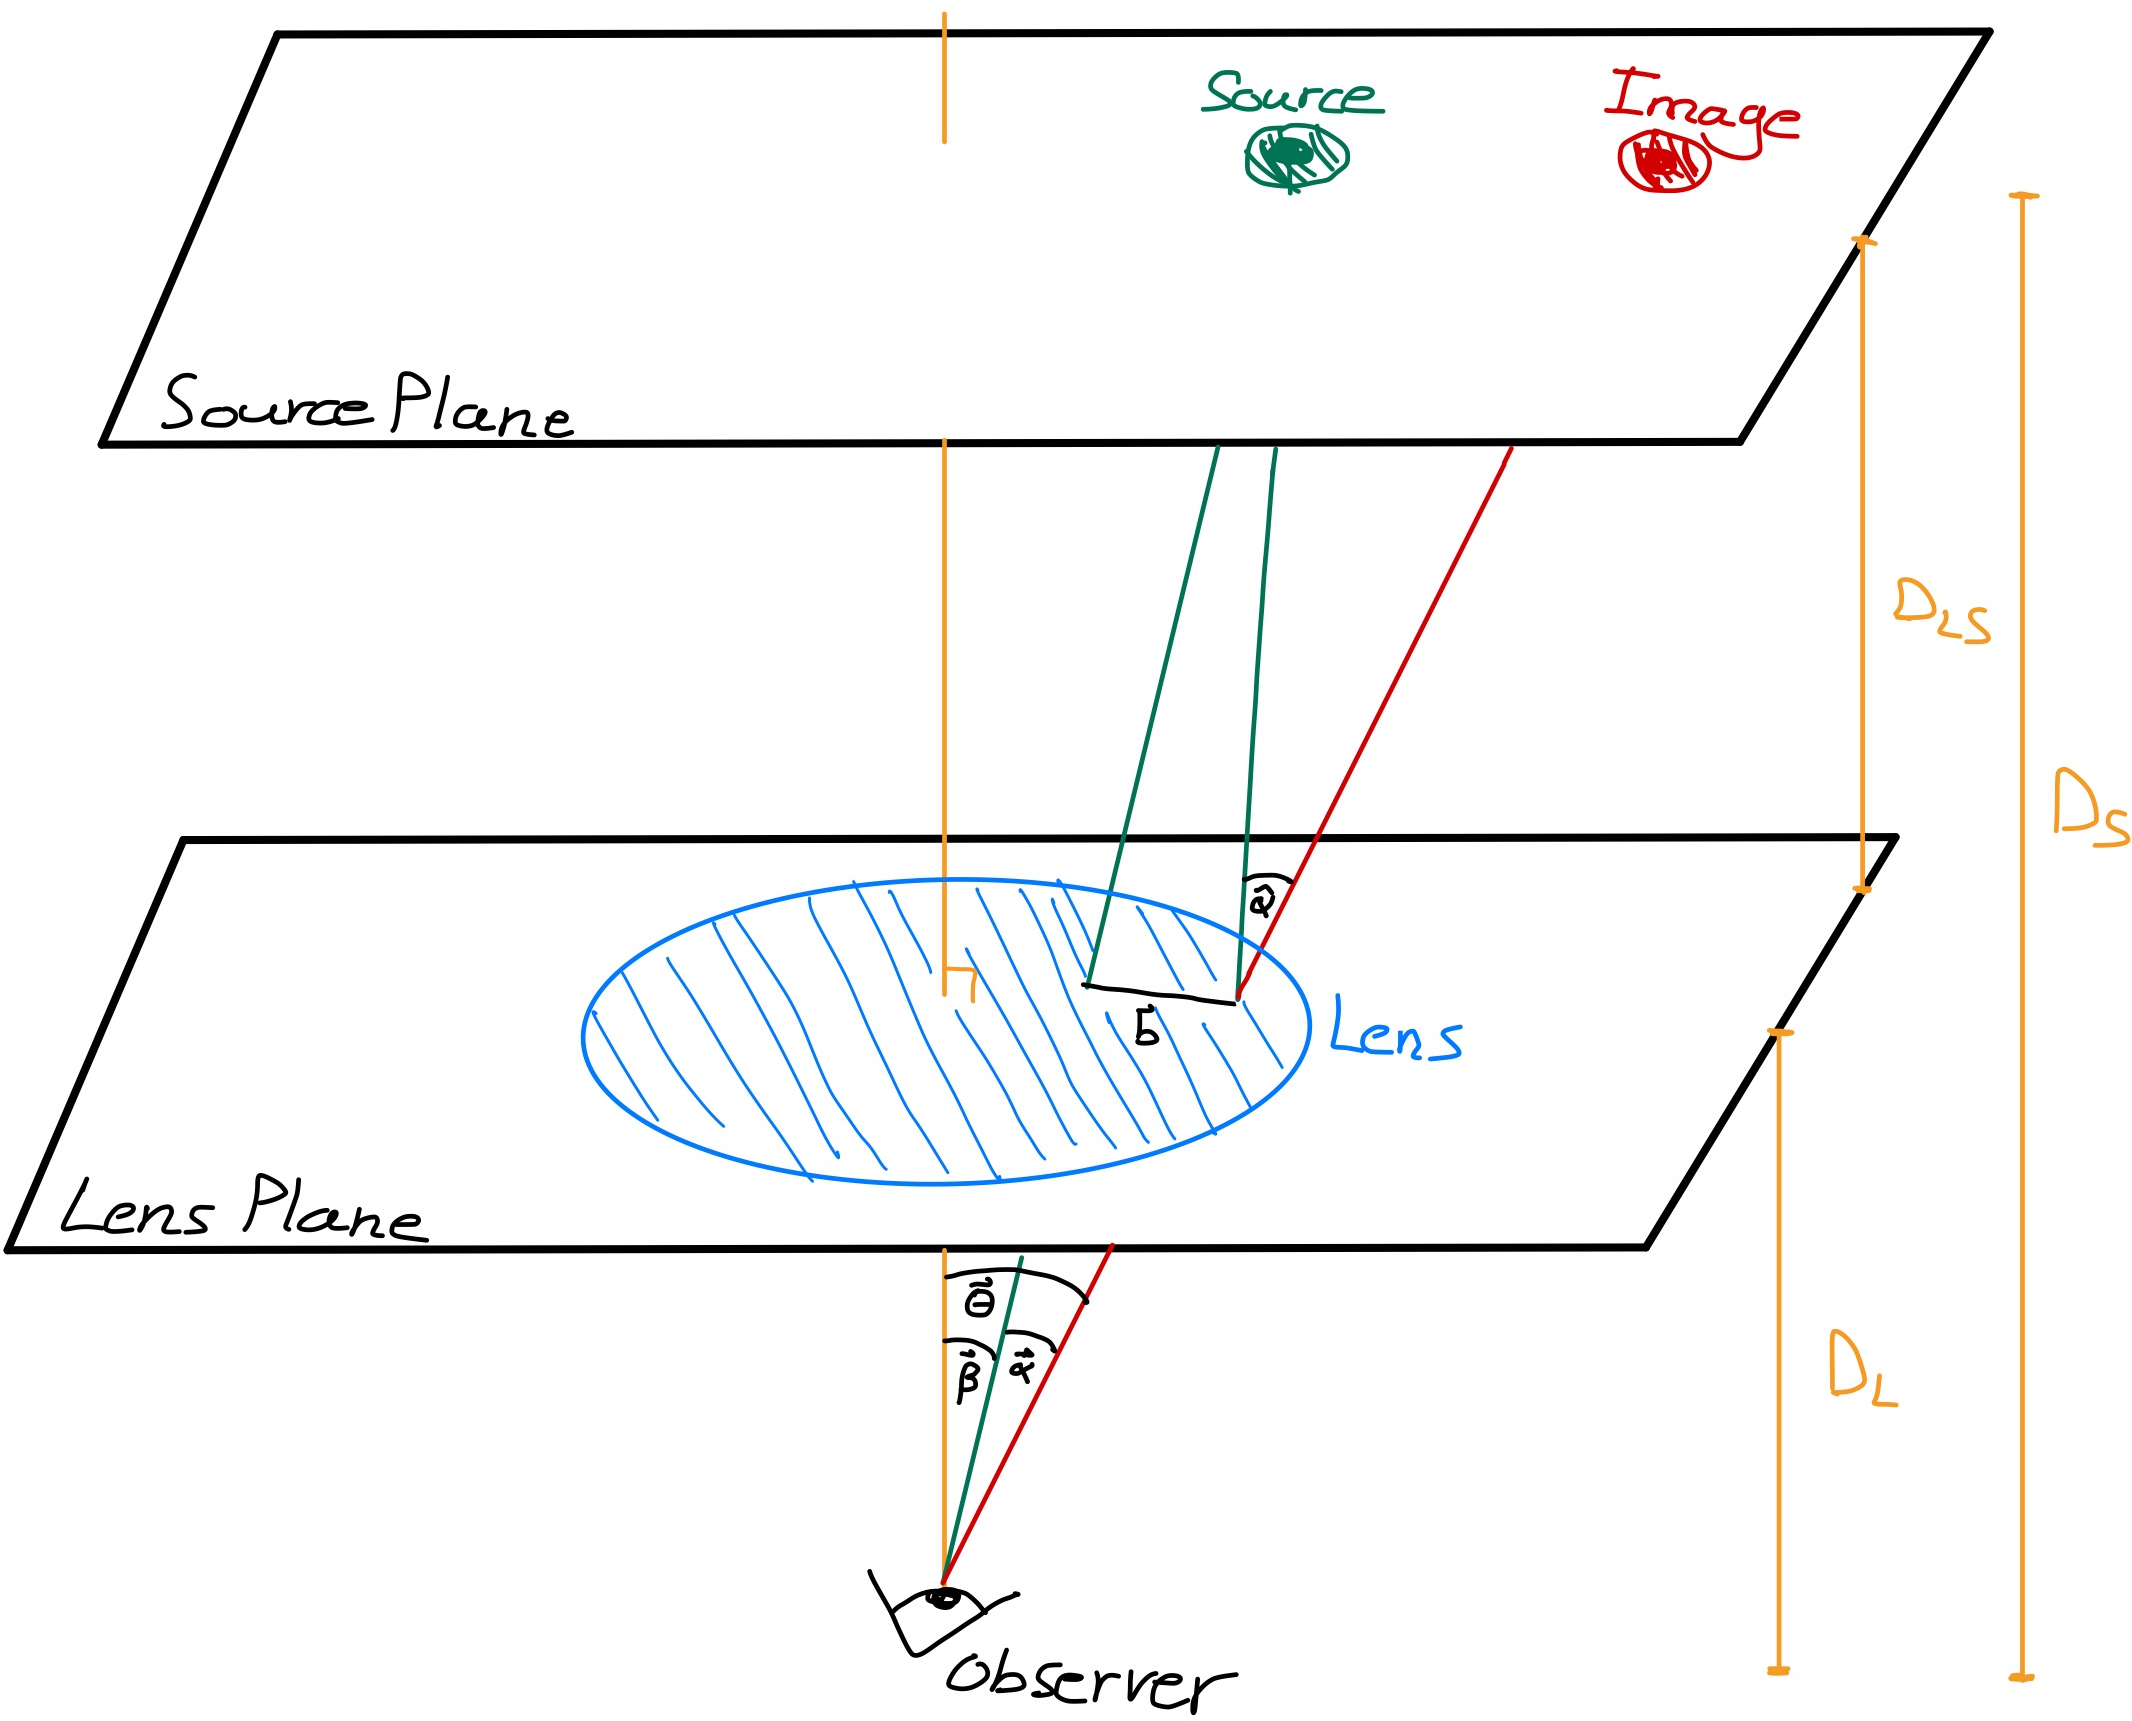
\includegraphics[width=\textwidth]{WeakLensing/figs/lens.jpg}
  \end{center}
  \caption{Sketch of a thin lens system highlighting the parameters of relevance in the weak lensing formalism. It is conventional to assume the planes are orthogonal to the z axis.}
  \label{fig:lens}
\end{figure}
In order to develop our formalism let us consider a general lensing system as seen in \autoref{fig:lens}. For astronomical applications on cosmological scales the distance from the observer to the lens $D_L$, the distance from the lens to the source $D_{LS}$, and the distance from the observer to the source $D_S$ are much greater than the thickness of the lens along the optical axis. Therefore we can treat the lens as a "thin lens", i.e. it lives on a planar slice (lensing plane) along the line of sight. We project the mass and potential of the lens onto the lensing plane by defining the projected surface density $\Sigma$ and projected potential $\Phi$ as

\begin{equation}
  \begin{split}
    \Sigma(x,y) &= \int \rho(x,y,z) dz \\
    \Phi &= \int \phi dz
  \end{split}
  \label{eq:surfacedensity+surfacepot}
\end{equation}

were $\rho$ and $\phi$ are the spatial mass density and the newtonian potential respectively. We can now use the results from the previous section to find the deflection angle $\hat{\alpha}$ due to the extended thin lens. The deflection is given by

\begin{equation}
  \hat{\alpha} = \frac{2}{c^2} \nabla \Phi(x,y)
  \label{eq:deflectionthinlens}
\end{equation}

were the factor of 2 comes from \autoref{grbend} and $\nabla$ is the two dimensional gradient. Note that this equation is equivalent to that describing the deflection of light by an optical lens with refractive index $n=1-2\Phi/c^2$, hence the name lensing. Geometrically we have $\beta = \theta - \alpha$ and $\hat{\alpha} = \frac{D_{LS}}{D_S}\alpha$ from \autoref{fig:lens}. This leads us to the ray trace equation

\begin{equation}
  \beta = \theta - \frac{D_{LS}}{D_S} \hat{\alpha}(\theta)
  \label{eq:raytrace}
\end{equation}

The ray trace equation is the fundamental equation in weak lensing relating all the geometric properties of the system to one another. 

\subsubsection{Differential deflection of adjacent light rays}
In the weak limit the actual deflections are not observable because the true position of the source is unknown. As a result, only the effects of differential deflection can be measured. Two adjacent light rays from the source pass through the lens at slightly different positions and will therefore be deflected differently. This effect results in a remapping of the observed surface brightness of the source $I_s$ to the observed surface brightness $I_{obs}$. This mapping can be linearized and is therefore given by 

\begin{equation}
  I_{obs}(\vec{\theta}) \approx I_s(A\vec{\theta})
  \label{eq:linearizedbright}
\end{equation}

were $A$ is the Jacobian of the transformation. A convenient convention is to rewrite the 2D Jacobian as 

\begin{equation}
  A = \delta_{ij} - \frac{\partial^2 \Phi}{\partial \theta_i \partial \theta_j} =  \begin{pmatrix}
    1-\kappa-\gamma_+ & -\gamma_\times \\
    -\gamma_\times & 1-\kappa+\gamma_+
    \end{pmatrix}
  \label{eq:Ajacobian}
\end{equation}

were we have defined the convergence $\kappa$ shear $\gamma = \gamma_+ + i \gamma_\times$ as 

\begin{equation}
  \begin{split}
   \kappa &= \frac{1}{2}(\partial_x^2 \Phi + \partial_y^2 \Phi)\\
   \gamma_+ &=  \frac{1}{2}(\partial_x^2 \Phi - \partial_y^2 \Phi)\\
   \gamma_\times &=  \partial_x \partial_y \Phi \\
  \end{split}
  \label{eq:kappagamma}
\end{equation}

We can now study the geometric implications of the remapping. If we consider a circular source we see that  $\gamma_+$ and $\gamma_\times$ correspond to a stretching of the circle along the x/y axis and the x=y line respectively, $\kappa$ corresponds to isotropic enlargement of the source's profile, and since the mapping conserves surface brightness we observe an increase of the total flux by a magnification factor

\begin{equation}
  \mu = \frac{1}{\text{det}A} = \frac{1}{(1-\kappa)^2 - \gamma_+^2 - \gamma_\times^2}
  \label{eq:magnificaiton}
\end{equation}

these geometric effects are illustrated in \autoref{fig:shears}. To be more specific a circular source is mapped to an ellipse with major axis $a = (1-\kappa - |\gamma|)^{-1}$ and minor axis $b = (1-\kappa + |\gamma|)^{-1}$ \cite{massey_2013}. If we define the reduced shear as $g = \gamma / (1-\kappa)$ then an ellipse with ellipticity $\epsilon_{orig}$ is mapped to an ellipse with ellipticity $\epsilon_{obs}$ given by 

\begin{equation}
  \epsilon_{obs} = \frac{\epsilon_{orig} + g}{1+g^* \epsilon_{orig}} \approx \epsilon_{orig} + \gamma
  \label{eq:ellip}
\end{equation}

the approximate relationship is a result of the weak limit ($\kappa << 1$). \autoref{eq:ellip} and \autoref{eq:kappagamma} demonstrate that by measuring the apparent shapes of lensed objects we are measuring information about the lensing potential and hence the matter overdensity \cite{rachel_2018,Hoekstra:2013gua,hoekstra}. \autoref{eq:ellip} indicates that a population of intrinsically round sources ($\epsilon_{orig}=0$) would be ideal, but unfortunately real  galaxies  have  an  average  intrinsic ellipticity of 0.25 per component \cite{Hoekstra:2013gua}. Instead the lensing signal is inferred by averaging over an ensemble of sources, under the assumption that the unlensed orientations are random \cite{rachel_2018,Hoekstra:2013gua}. In the next section we talk about how such measurements are made.

\begin{figure}
    \begin{center}
      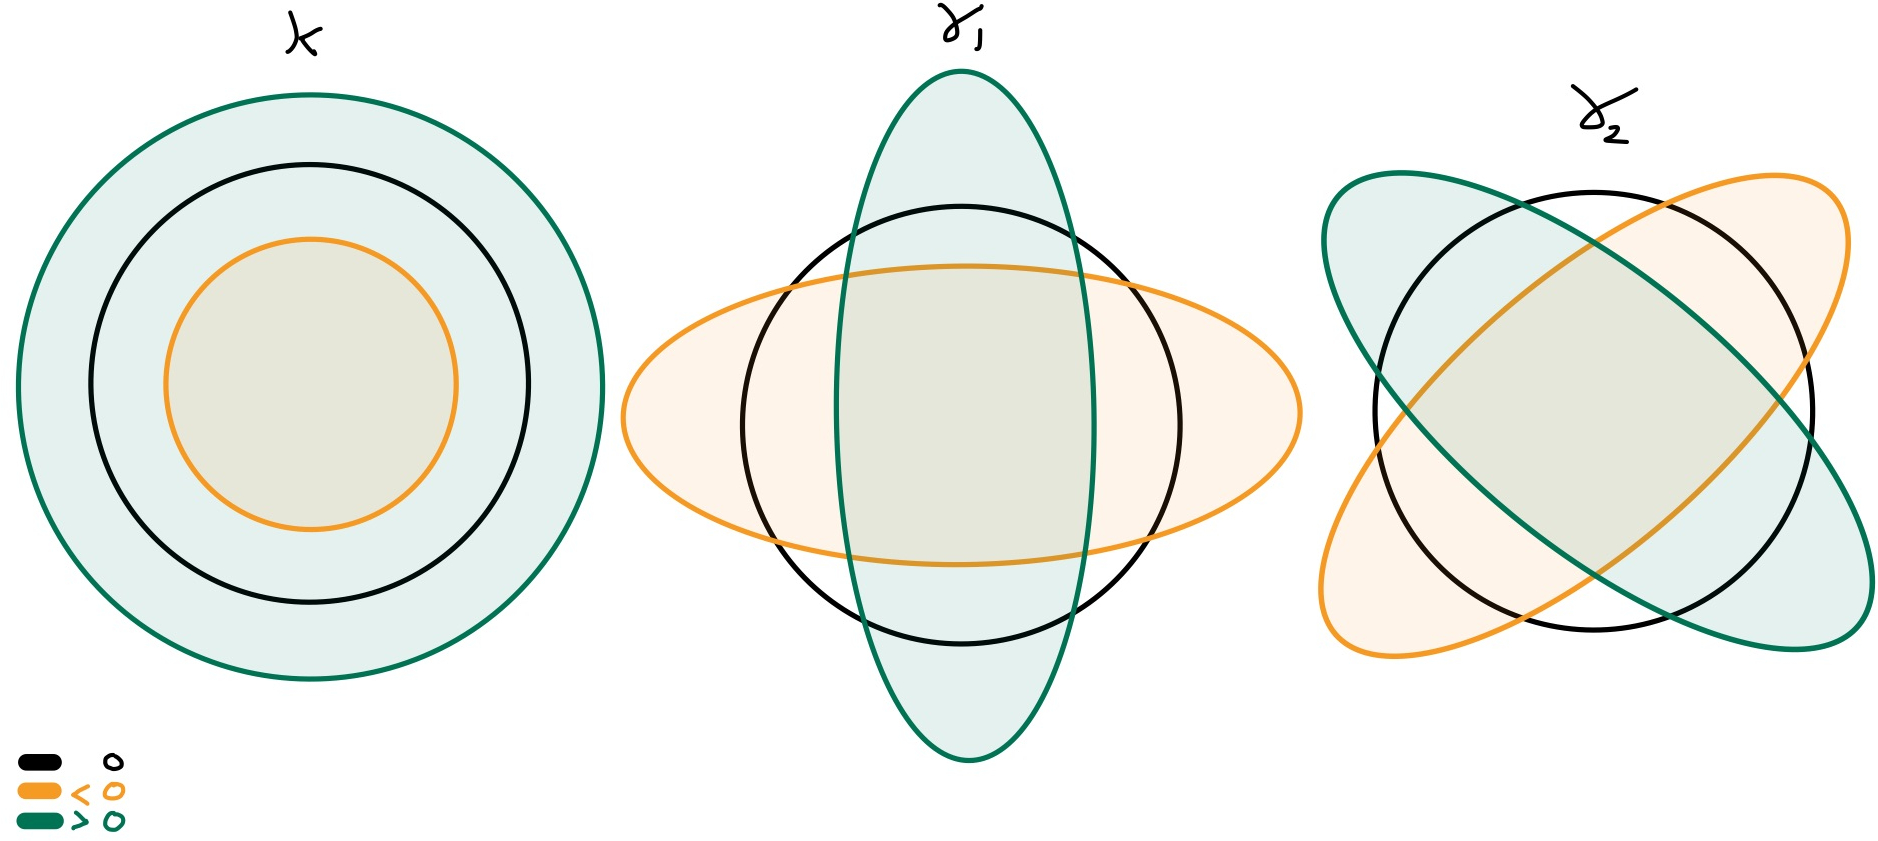
\includegraphics[width=\textwidth]{WeakLensing/figs/shear-11.jpg}
    \end{center}
    \caption{The effects of the convergence $\kappa$ and  the shear $\gamma$ on a circular image of a galaxy. The black line represents the nominal image, orange represents positive parameter values, and green represents negative parameter values.}
    \label{fig:shears}
\end{figure}

% Cosmology standard model and lensing formalism
% begin{enumerate}
%     \item Current observations imply w=-1 however that is no constraint on its evolution
%     \item The inital fluctation ins matter density produced by random quantum events therefore CLT tells us that is a gaussiam random field therefore power spectrum is enough to get all statistics
% \end{enumerate}


\section{Measuring Shear (Images to Catalogs)}
The weak lensing analysis process can be conceptually split into two parts; 1) converting images to catalogs of galaxy shapes and 2) extracting scientific results from shape catalogs. In this section we present a sample image to catalog pipeline. An overview of a weaklensing analysis pipeline is presented in \autoref{fig:pipe}.

\begin{figure}
    \begin{small}
        \begin{center}
            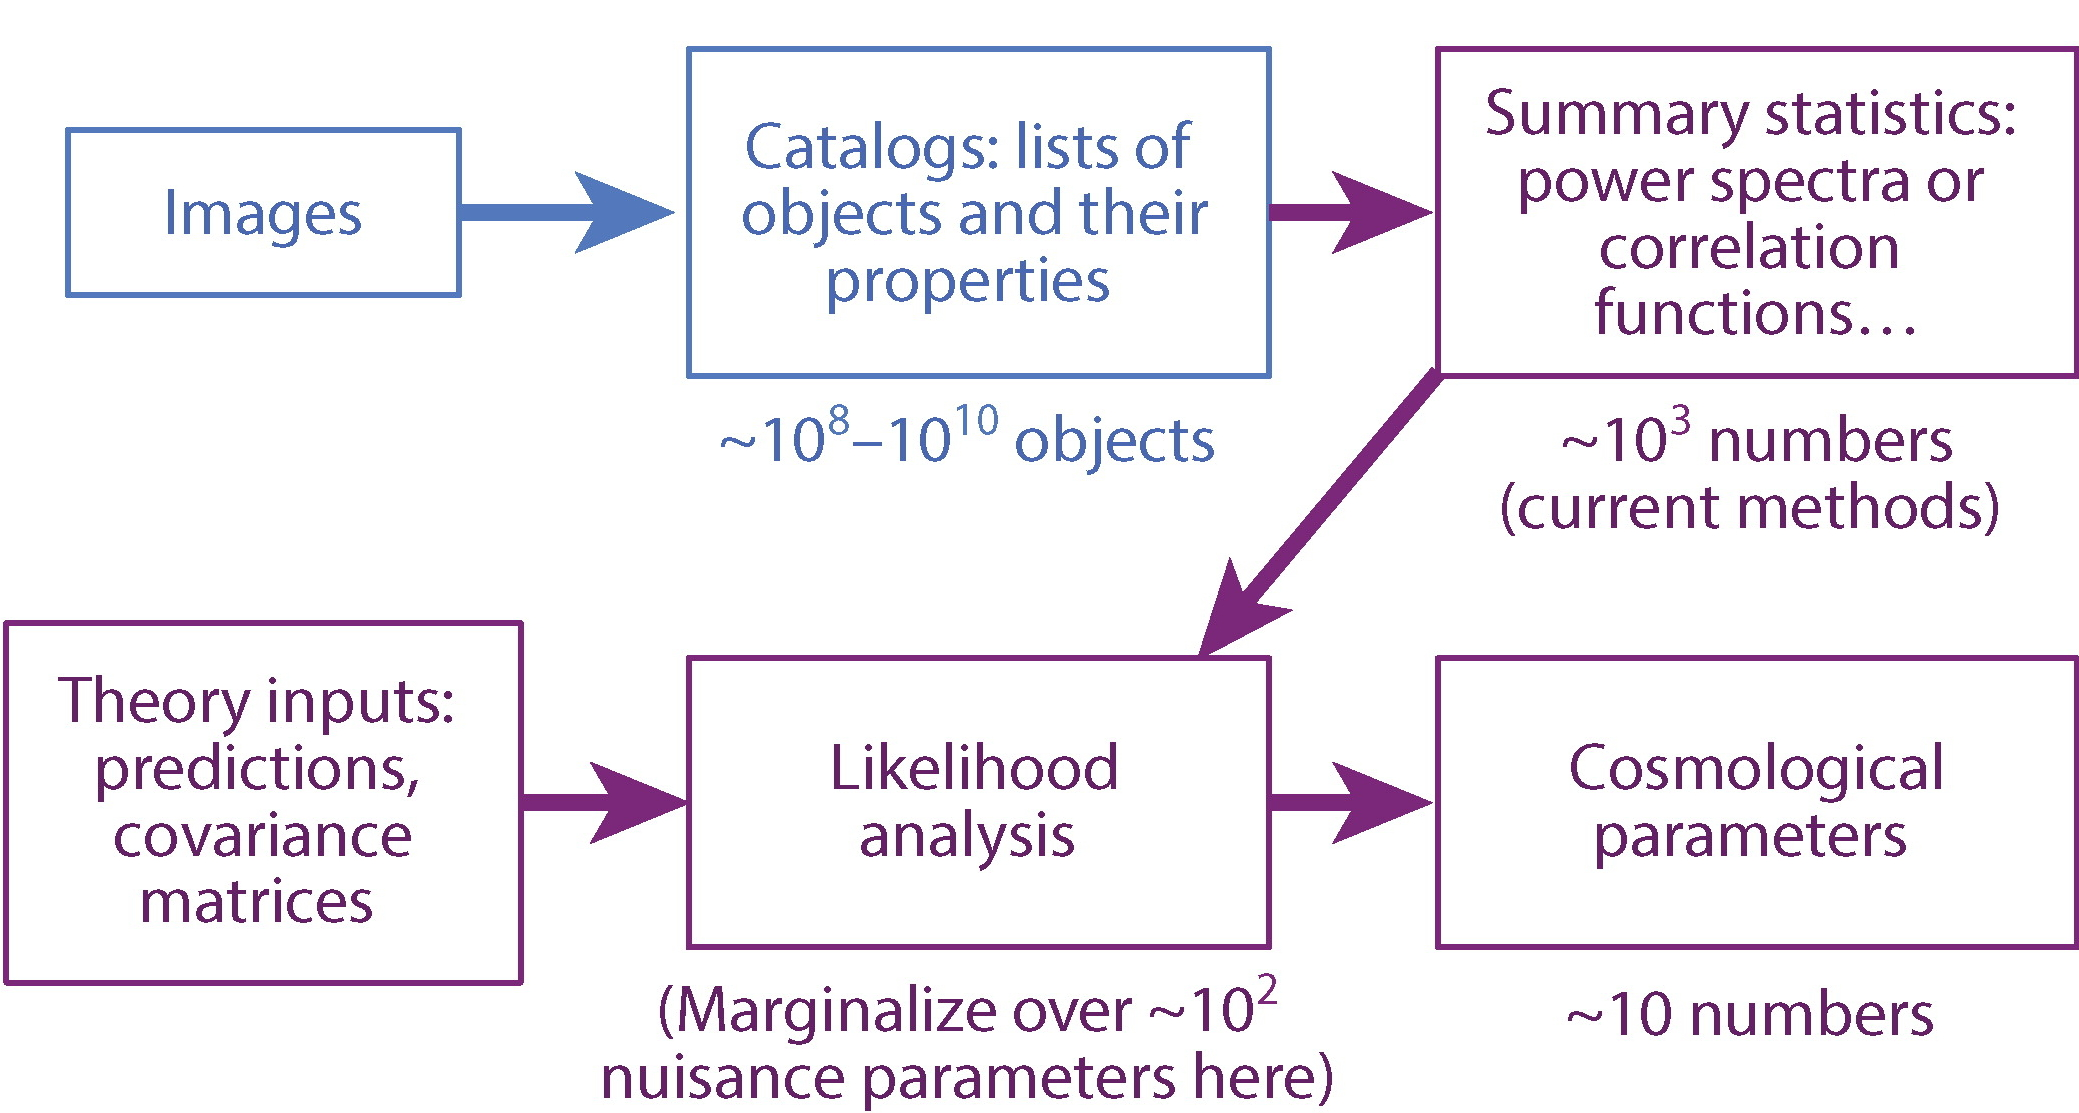
\includegraphics[width=0.95\textwidth]{WeakLensing/figs/pipe.jpg}
        \end{center}
        \caption{A generic outline of weak lensing pipeline analysis as presented in \cite{rachel_2018}. Note this is a cosmic shear pipeline and therefore is not identical to what a SuperBIT pipeline would look like. In the case of cluster count applications an additional block of mass calculations would be needed.}
        \label{fig:pipe}
    \end{small}
\end{figure}


\subsubsection{Object Detection}

The first step in weak lensing analysis is to detect the objects that will be analyzed. In the case of cosmological data the objects of interest are faint distant galaxies. Traditional methods for galaxy detection simply involve the detection of peaks above some detection threshold in a long exposure image. However due to the subtlety of the weak lensing signal the process is more involved. First we must confidently distinguish stars from galaxies, this is a fairly straight forward process that is usually done with photometric data. The next step is to detect galaxies that have blended together in the imaging process, i.e. detections with a double peak feature. Such blended images account for upto 10\% of detections and therefore need to be either deblended or discarded from the data set \cite{rachel_2018,general_2013}. Finally, based on the systematics of the detector some selection criteria is introduced that will filter out problematic images. 

\par Alternatively, another way galaxies are detected in images is by a likelihood analysis comparing imaged brightness profiles $I$ to theoretical brightness profiles predicted by galactic theories.

\subsubsection{Shape Extraction}
After the galaxies are detected their shapes need to be measured. The accurate measurement of galaxy shape from an image is a rich and complex topic, we will state some results from \cite{massey_2013,general_2013} without derivation. Galaxy shapes can be quantified by computing the second moments of the galaxy images 

\begin{equation}
    Q_{ij} = \frac{\int  d^2x I(\vec{x}) W(\vec{x})x_ix_j}{\int d^2x I(\vec{x}) W(\vec{x}) }
    \label{eq:moments}
\end{equation}


were $I$ is the brightness profile defined in \autoref{eq:linearizedbright} and $W$ is a weighting function introduced to effectively limit the domain of the integral. The exact relationship between the the second moments and ellipticity is convention dependant, in this section we will use the same definitions as \cite{rachel_2018,Hoekstra:2013gua}. The size $R$ and complex ellipticity $\epsilon$ are given by

\begin{equation}
    R^2 = Q_{11} + Q_{22}
    \label{eq:size}
\end{equation}

\begin{equation}
    \epsilon = \frac{Q_{11}-Q_{22}+2iQ_{12}}{Q_{11}+Q_{22}}
    \label{eq:ellipticity}
\end{equation}

All ellipticity definitions have a well-defined response to a lensing shear and, hence, recover the same science after averaging across ensembles of galaxies. \autoref{eq:ellip} tells us that averaging over a randomly oriented galaxies gives us the mean shear ($\left< \epsilon \right > = \left< \epsilon_{orig}\right> + \left<\gamma \right> = \left<\gamma \right>$) and therefore an accurate measurement of $\epsilon$ suffices for statistical analysis. 

\par Note that if the alternative object detection method is used, i.e. model fitting, then the ellipticity can be simply read off the best fit model without the need for computing second moments.

\subsubsection{Point Spread Function}
The point spread function (PSF) describes the response of an imaging system to a point source or point object. In practice the surface brightness profile of an object in an image is not the $I_{obs}$ from \autoref{eq:linearizedbright} but is convoloved with some unknown function $PSF(\vec{x})$. Therefore, in order to detect weak lensing signal we must understand and reconstruct our PSF in order to deconvolve it from the image. Deconvolving the PSF is the most important and most difficult step of any weak lensing analysis \cite{Hoekstra:2013gua,rachel_2018}. The PSF has a width which leads to rounder images and typically is anisotropic, which leads to a preferred orientation. The bias is grouped into two kinds: a multiplicative bias $m$ that scales the shear, and an additive bias $c$ that reflects preferred orientations that are introduced. The observed shear and true shear are thus related by

\begin{equation}
    \gamma_{obs} = (1+m) \gamma + c
     \label{eq:shearobs}
\end{equation}

In order to take this effect the PSF must be accurately estimated and deconvolved from the results. This is done by observing a large field of stars and recording the optical systems response to a star as a function of position. The function is then estimated by interpolating between star positions.



\section{Catalogs to Science}
After we have measured galaxy shapes to the necessary accuracy we need to extract cosmological results from the data. More specifically we want to be able to extract the density contrast power spectrum discussed in the Section 2. 

\subsection{Convergence Power Spectrum}
We first note that in the weak limit we can use the 3D newtonian comoving poisson equation

\begin{equation}
    \nabla^2 \phi = \frac{3H_0 ^2\Omega_m }{2a} \delta
    \label{eq:poisson}
\end{equation}

were $\delta$ is the density contrast defined in \autoref{eq:densitycontrast}. Therefore, we can rewrite the convergence as

\begin{equation}
    \kappa = \frac{3H_0^2}{2c^2} \Omega_m \int_{0}^{\chi_s} d\chi  \frac{\chi (\chi_s-\chi)}{\chi_s} \frac{\delta(\chi)}{a}
    \label{eq:kappadelt}
\end{equation}

were $\chi$ is the comoving angular diameter distance and $a$ is the scale factor. \autoref{eq:kappadelt} shows that the convergence is a projection of the density contrast with the weight function 

\begin{equation}
    w(\chi) = \frac{3H_0^2 \Omega_m \chi (\chi - \chi_s)}{2 c^2 \chi_s a}
    \label{eq:weight}
\end{equation}

thus, the convergence power spectrum is determined by the integral over the line of sight of the density contrast power spectrum\cite{Hoekstra:2013gua,rachel_2018,Bartelmann:2016dvf}. More specifically, the convergence power spectrum can be written using the parameters from \autoref{eq:powerspecd} as 

\begin{equation}
    C_\kappa(l) = \frac{9}{4} \left(\frac{H_0}{c}\right)^4\Omega_m^2 \sigma_8^2 \int^{\chi_s}_0 d \chi \left[\frac{G(t)\chi (\chi_s-\chi)^2}{a \chi_s}\right] \mathcal{P}\left(\frac{1}{\chi}\right)
    \label{eq:convergencespectrum}
\end{equation}

\autoref{eq:convergencespectrum} shows that the shape of $C_\kappa$ depends on the shape $\mathcal{P}$ of the density contrast power spectrum and thus can be inferred from a measurement of the convergence power spectrum. The growth factor $G$ can also be measured to give us information of on the evolution of structure growth with time. Finally, while we set out to measure the influence of dark energy on structure formation \autoref{eq:convergencespectrum} allows us to additionally constrain the cosmological parameters $\Omega_m$ and $\sigma_8$ up to a degeneracy. The degeneracy is physically interpreted as weak lensing inability to differentiate between low density highly clumped matter and weakly clumped high density matter \cite{general_2013,Bartelmann:2016dvf}. 

\subsection{Cosmic Shear}
In the previous subsection we showed that if we could measure the convergence power spectrum then we will have achieved our scientific goal. However, you might notice that we never discussed measuring convergence, we only explained shear measurements. The reason is that measuring the convergence is significantly more challenging than measuring the shear. But, it turns out that the convergence power spectrum is identical to shear power spectrum, therefore, our shear data suffices. To prove the statement let us begin by taking the fourier transform of \autoref{eq:kappagamma}, the result is 

\begin{equation}
    \begin{split}
        2\hat{\kappa} &= -l^2 \hat{\Phi} \\
        2 \hat{\gamma}_+ &= -(l_1^2-l_2^2) \hat{\Phi} \\
        \hat{\gamma}_\times &= -l_1l_2 \hat{\Phi}
    \end{split}
    \label{eq:fouriertrans}
\end{equation}

were the hat indicates the fourier transform of the function. \autoref{eq:fouriertrans} allows us to investigate the magnitude of the functions, we find that

\begin{equation}
    4|\hat{\gamma}| = |\hat{\Phi}|^2 \left(l_1^2+l_2^2\right)^2 = 4 |\hat{\kappa}|^2
    \label{eq:fourierspace}
\end{equation}

The power spectrum of a gaussian field depends exclusively on the magnitude therefore \autoref{eq:fourierspace} shows that the shear power spectrum $C_\gamma$ is the same as the convergence power spectrum $C_\kappa$ \cite{Bartelmann:2016dvf,Hoekstra:2013gua,rachel_2018,general_2013}. The shear power spectrum is simply the fourier transform of the two point correlation function given by 

\begin{equation}
    \xi_{ij} = \left< \gamma_i \cdot \gamma_j^*\right> 
    \label{eq:2ptcorrelation}
\end{equation}

were $i$ and $j$ are redshift bin indices. This two point correlation is the so called "cosmic shear" and is physically the correlation between shears separated by an angular mode on the sky, i.e. if some image distortion by lensing is measured in one particular direction the image distortion nearby should be more similar and thus more correlated than a distortion far away. For a more in depth discussion on cosmic shear please see \cite{lensingbook,general_2013,Hoekstra:2013gua,Bartelmann:2016dvf}.

 \par The above discussion is the extraction procedure for ideal data. Working with real data is more challenging and requires the development of more tools, due to report size constraints we will not be presenting any further analysis techniques.

 \subsection{Sunyaev-Zeldovich Cluster Count}
 hi


\section{Weak Lensing Results}
Some weak lensing results are already available from collocations such as DES and Subaru. These results include measurements of the power spectrum, contour constraint plots of $\Omega_m$ and $\sigma_8$, and tomogrophic data of the powers pectrum as a function of redshift. The results can be found in \cite{Subaru_2019}.

\section{Systematics}
Finally, we end this report with a discussion with a topic almost synonymous with weak lensing, systematic errors. Weak lensing has proven the most technically challenging cosmological probe due to the large range of systematic errors it suffers from \cite{general_2013}. Below We present a very brief overview over the rich topic of weak lensing systematics, for more details please see \cite{massey_2013,general_2013}.

\begin{enumerate}
    \item \textbf{PSF Errors:} As mentioned previously the PSF of the optical system needs to be estimated in order to extract meaningful data. This estimation involved interpolation between the systems response to a star, this interpolation is a less accurate representation of the PSF the further we get from a star. This uncertainty in the PSF could result in systematically introducing additional shear in a subset of the data and therefore detecting false signals. 
    \item \textbf{Blending:} As discussed previously approximately 10\% of the galaxies observed have some form of blending. This introduces the following problem; we can be over aggressive with our blended object identification which could result in non blended objects being flagged as blended and unnecessarily tampered with or conversely we could be too lenient with our detection allowing blended objects into our analysis. Both cases would introduce a systematic error into our data. Additionally, even if our detection algorithm is perfect our deblending algorithm might not be which would induce a systematic in 10\% of the data.
    \item \textbf{Selection Bias:} Depending on the optical system used to detect the galaxies an algorithm is needed to filter out unusable objects. The reason an object is unusable could stem from PSF uncertainty, blending, detector systematics or any other reason. Imperfections in such algorithms could result in an implicit shape dependance on the selection, such a dependance introduces/removes shear signal from the data.
    \item \textbf{Intrinsic Alignment:} Finally, throughout this entire the report the fundamental assumption as been that galaxy orientations are randomly distributed. This assumption is not entirely true, factors such as proximity to other galaxies, angular momentum during formation, and location relative to the center of mass of a cluster all impact the alignment of galaxies. A good example of this is the fact that galaxies near the center of a cluster tend to be oriented in a manner such that they point towards the center\cite{rachel_2018}.
\end{enumerate}

